\section{System Description}
DBIE is designed to run on Linux and its operability has been confirmed on
Ubuntu. The following sections detail various design choices made during the
implementation of DBIE.
%
\subsection{Basic Terminology}
A \term{node}---as it relates to our system---is a single computer that can
operate independently. A \term{process} is an instance of a program that is
being executed; each process contains the program code and the memory in use by
the current execution.
\subsection{Client}
Our system's ``client'' is a database management system (DBMS). The DBMS
interfaces with our system through two actions: \code{PUT} which adds data to
the system (or updates existing data), and \code{QUERY} which requests the
results of a given query on the index. In production, the DBMS could be a
full-featured product like SQLite, but we created a faux DBMS that provided
fine-grained control for our testing.
%
\subsection{System Structure}
The two most established structures for a distributed system are the
master-slave model and the peer-to-peer model; in both cases, let us assume we
have \(N\) total nodes. In both models, a client (be it a person, another
system, etc.) makes a request of the system and will expect some sort of
response (a result, an acknowledgment, etc.). In the peer-to-peer model each of
the \(N\) peers can accept requests and then delegate work to their peers. Once
the request has been satisfied, whichever peer has the final result will return
the result to the client. In the master-slave model there exits a single
``master'' node and \(N - 1 = n\) ``slave'' nodes. The master node accepts
requests and then delegates the work to the slaves which return results to the
master which will in turn return the final result to the client. We chose to
structure our system using the master-slave model instead of the peer-to-peer
model because it is a very intuitive way of structuring the query problem.
Further, we chose to use a \term{replication factor} of two---i.e., each piece
of data is stored on two separate nodes---when distributing data to the slaves.
%
\subsection{Communication}
Distributed systems require additional methods of communication beyond those
used in single-process or even single-node systems. Communication between nodes
was accomplished using remote procedure calls (RPCs). An RPC is simply a
function call from one process to another \cite{tanenbaum1994}. RPCs are a
method of simplifying communication between nodes by hiding the networking
details and instead allowing developers to make function calls between nodes.
This helps to make the source code more readable and avoid mistakes in manually
opening and closing network connections.
%
\subsection{Bitmap Compression}
In order to perform the necessary bitmap operations (\code{AND}s and
\code{OR}s), we utilized Chiu et al.'s bitmap engine which had been developed
by several students under the direction of Professor David Chiu. Chiu et al.'s
bitmap engine has implemented three compression and query methods: Byte aligned
Bitmap Code (BBC), Word aligned Hybrid Code (WAH), and Variable aligned Length
Code (VAL). Each of these three compression and query methods provides
substantial benefits over the use of uncompressed bitmap vectors. Of the three,
we chose to use WAH as it has been shown to be faster than BBC and it has a
simpler formatting than VAL. WAH allows compression of vectors such that all
information the vector gives is encoded, allows compressed vectors to be
queried. A complete description of WAH is given by \cite{wu2001}.
%
\subsection{Consistent Hashing}
To determine on which two machines a given vector is located (or should be
located, if the identifier is new to the system) we use an algorithm known as
consistent hashing. Consistent hashing was introduced by
Karger~et~al.~\cite{karger1997} and can be understood conceptually as follows.
\par
Each slave machine is assigned a point on a circle where each point corresponds
to a value between \(0\) and \(2^{64} - 1\). The point for a machine with
identifier \(i\) is calculated as
\begin{equation*}
    \func{h}{i} \coloneqq \func{SHA1}{i} \bmod{2^{64}}.
\end{equation*}
To determine which machines (should) contain the vector \(k\), walk clockwise
from the point \(\func{h}{k}\) until reaching a machine node (the
\term{primary} node), and keep walking until reaching the next machine node
(the \term{backup} node). Once the primary and backup nodes have been
determined, return the set comprised of those two nodes. This process is
represented visually in Figure~\ref{fig:ring-hash-process} and formalized in
Algorithm~\ref{alg:consistent-hashing}.
%
\par
In our system, the consistent hashing structure is maintained as a red-black
tree, and the process of determining the next node is given by the algorithms
\procedure{Tree-Succ} (Algorithm~\ref{alg:tree-succ}) and
\procedure{Recur-Succ} (Algorithm~\ref{alg:recur-succ}). When the system is
initialized, each machine is assigned a nonnegative integer as an identifier.
After the identifiers are assigned, they are inserted into the tree. Each node
has pointers to its left child, right child, and parent (accessible via the
functions \procedure{Left}, \procedure{Right} and \procedure{Par},
respectively). If a node does not have a parent or a child, that pointer will
hold the value \(null\). The algorithms for \procedure{Tree-Min} and
\procedure{Tree-Max} are given in \cite{cormen2009}
%
\begin{algorithm}
    \begin{algorithmic}
        \Procedure{Recur-Succ}{$tree, root, succ, key$}
            \If{$root = null$}
                \State \Return $succ$
            \ElsIf{$key = \func{h}{root.id}$}
                \State $succ \gets \Call{Right}{root}$
                \If{$succ = null$}
                    \State $succ \gets root$
                    \While{$\Call{Par}{succ} \neq null \land \func{h}{succ} < key$}
                        \State{$succ \gets \Call{Par}{succ}$}
                    \EndWhile
                \Else
                    \While{$\Call{Left}{succ} \neq null$}
                        \State{$succ \gets \Call{Left}{succ}$}
                    \EndWhile
                \EndIf
                \Return {$succ$}
            \ElsIf{$\func{h}{root.id} > key$}
                \State $left \gets \Call{Left}{root}$
                \State \Return \Call{Recur-Succ}{$tree, left, root, key$}
            \Else
                \State $right \gets \Call{Right}{root}$
                \State \Return \Call{Recur-Succ}{$tree, right, succ, key$}
            \EndIf
        \EndProcedure
    \end{algorithmic}
    \caption{Recursively Determined Successor Node}
    \label{alg:recur-succ}
\end{algorithm}
%
\begin{algorithm}
    \begin{algorithmic}
        \Procedure{Tree-Succ}{$tree, key$}
            \If{$\func{h}{key} \geq \func{h}{\Call{Tree-Max}{tree}.id}$}
                \State \Return \Call{Tree-Min}{$tree$}
            \Else
                \State $root \gets \Call{Root}{tree}$
                \State \Return \Call{Recur-Succ}{$tree, root, root, key$}
            \EndIf
        \EndProcedure
    \end{algorithmic}
    \caption{Successor Node \cite{bstPredecessorSuccessor}}
    \label{alg:tree-succ}
\end{algorithm}
%
\begin{algorithm}
    \begin{algorithmic}
        \Procedure{Consistent-Hash}{$tree, key$}
            \State $m_0 \gets \Call{Tree-Succ}{tree, key}$
            \State $m_1 \gets \Call{Tree-Succ}{tree, m_0.id}$
            \State \Return $\set{m_0, m_1}$
        \EndProcedure
    \end{algorithmic}
    \caption{Consistent Hashing}
    \label{alg:consistent-hashing}
\end{algorithm}
%
\begin{figure}
    \centering
    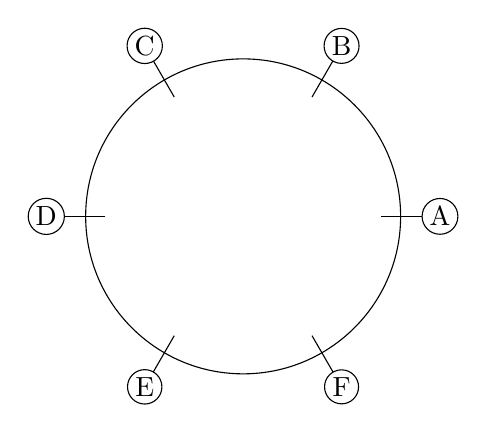
\begin{tikzpicture}
    \draw (0,0) circle (2);
    \draw (0:1.75) -- (0:2.5) node [draw, shape=circle, inner sep=1, fill=white, text=black] {A};
    \draw (60:1.75) -- (60:2.5) node [draw, shape=circle, inner sep=1, fill=white, text=black] {B};
    \draw (120:1.75) -- (120:2.5) node [draw, shape=circle, inner sep=1, fill=white, text=black] {C};
    \draw (180:1.75) -- (180:2.5) node [draw, shape=circle, inner sep=1, fill=white, text=black] {D};
    \draw (240:1.75) -- (240:2.5) node [draw, shape=circle, inner sep=1, fill=white, text=black] {E};
    \draw (300:1.75) -- (300:2.5) node [draw, shape=circle, inner sep=1, fill=white, text=black] {F};
\end{tikzpicture}

    \caption{Visualization of Ring Consistent Hashing}
    \label{fig:ring-hash-process}
\end{figure}
%
\subsection{Consistency}
After we had decided on a method for determining \emph{where} to store data,
we needed a method of ensuring that the data actually arrived at each node it
was suppose to. To do this, we implemented a system called Two-Phase Commit
(TPC) which ensures data consistency. It does this by checking that both slaves
are available: if so, the data is sent to both, if either is unavailable, the
unavailable node is handled and the process is restarted.
%
\subsection{Fault Tolerance}
The primary reason for using consistent hashing is for fault tolerance. While
waiting for messages from the DBMS, the master pings each slave to ensure that
each slave node is still online. If it doesn't hear back from a slave after a
reasonable length of time (one second in our system), it assumes that slave is
out of commission, and reallocates the vectors using \procedure{Reallocate}
(Algorithm~\ref{alg:reallocate}). To each node in the tree we store the set of
vectors that map to this machine, specifically for this purpose.
%
\begin{algorithm}
    \begin{algorithmic}
        \Procedure{Reallocate}{$tree, slave$}
            \State{$pred\gets\procedure{Tree-Pred}(tree, slave)$}
            \State{$succ\gets\procedure{Tree-Succ}(tree, slave)$}
            \State{$ssucc\gets\procedure{Tree-Succ}(tree, succ)$}
            \ForAll{$v\in (slave.vectors \cap succ.vectors)$}
                \State{$\procedure{Send-Vector}(succ, v.id, ssucc)$}
            \EndFor
            \ForAll{$w\in (slave.vectors \cap pred.vectors)$}
                \State{$\procedure{Send-Vector}(pred, w.id, succ)$}
            \EndFor
            \State{$\procedure{RB-Delete}(tree, slave)$}
        \EndProcedure
    \end{algorithmic}
    \caption{Reallocation}
    \label{alg:reallocate}
\end{algorithm}
%
\par
In our implementation we utilized algorithms provided by \cite{cormen2009}
to find the predecessor of a slave (\procedure{Tree-Pred}), to find the
successor of a slave (\procedure{Tree-Succ}), and to delete a slave from the
tree (\procedure{RB-Delete}). We also made use of an RPC,
\(\func{\procedure{Send-Vector}}{s_1, k, s_2}\),
that we wrote which makes slave \(s_1\) send the vector \(k\) to slave \(s_2\).
\par
As a result of using consistent hashing, we know that the failed slave's backup
vectors are the primary vectors of its predecessor. The successor must now
maintain copies of the predecessor's vectors, so the master tells the
predecessor to communicate its primary vectors to the successor. Likewise,
since the successor node now holds the slave's primary vectors alongside its
own, it must send the slave's primary vectors to its successor as a backup.
Consistent hashing is preferable to using a hash-mod-n or round-robin technique
because potentially every every single vector would have to be remapped,
requiring significantly more messages and more nodes involved than the ones
used in \procedure{Reallocate} to reconfigure the system. This is because for
hash-mod-n and round robin, algorithms whose hash function modulus is the
number of machines, when a slave node is removed, the primary locations of
potentially every vector changes, thus requiring us to remap every single
vector \cite{kleppman2017}. While hash-mod-n requires \(\func{O}{K}\)
remappings, where \(K\) is the number of keys, consistent hashing only requires
\(\func{O}{K/n}\), where \(n\) is the number of slaves
\cite{karger1997}.
%
\subsection{Queries}
Our system is designed to handle range queries. An example range query is
\code{R:[0,3]\&[5,7]}. Such a query might correspond to a range query in SQL.
The query given above requires the following steps:
\begin{algorithmic}
    \State $w_0 \gets v_0 \lor v_1 \lor v_2 \lor v_3$
    \State $w_1 \gets v_5 \lor v_6 \lor v_7$
    \State \Return $w_0 \land w_1$
\end{algorithmic}
To carry out the query, we first create a plan that tells us which slave nodes
to visit.
\subsection{Query Planning}
Our query planning algorithm (Algorithm~\ref{alg:query-planning}) takes two
inputs. The first input, \(tree\), is the red-black tree used in consistent
hashing to determine which two machines contain a given vector identifier. The
second input,
\[R = \set{\tuple{v_0, v_1}, \tuple{v_1, v_2}, \ldots, \tuple{v_n, v_m}},\]
holds the ranges of the query as an ordered set of tuples where
\(v_i \leq v_j\) and \(0 \leq i \leq j \leq n \leq m\), and each \(v_i\) is a
vector identifier. Sorting is performed so that, in each portion of the query,
slaves do not have to be visited more than once.
%
\begin{algorithm}
    \begin{algorithmic}
        \Procedure{Range-Query-Plan}{$tree, R$}
            \State{$swap \gets false$}
            \State{$paths \gets \emptyset$}
            \ForAll{$r \in R$}
                \State{$subpaths \gets \emptyset$}
                \For{$k \gets r_0, r_1$}
                    \State{$machines \gets \Call{Consistent-Hash}{tree, k}$}
                    \State{$tuple \gets \emptyset$}
                    \If{$swap$}
                        \State{$tuple \gets tuple \cup \set{machines_0}$}
                    \Else
                        \State{$tuple \gets tuple \cup \set{machines_1}$}
                    \EndIf
                    \State{$tuple \gets tuple \cup \set{k}$}
                    \State{$subpaths \gets subpaths \cup tuple$}
                \EndFor
                \State{Sort $subpaths$ on $machine.id$}
                \State{$paths \gets paths \cup subpath$}
                \State{$swap \gets \neg swap$}
            \EndFor
            \Return $paths$
        \EndProcedure
    \end{algorithmic}
    \caption{Query Planning}
    \label{alg:query-planning}
\end{algorithm}
%
\subsection{Query Execution}
Execution of queries received by the master is handled using
Algorithm~\ref{alg:master-query-root} which first plans out the query using
Algorithm~\ref{alg:query-planning} and then delegating work to the slaves using
Algorithm~\ref{alg:slave-subquery}.
%
\begin{algorithm}
    \begin{algorithmic}
        \Procedure{Master-Query-Root}{$Q$}
            \State $R \gets \emptyset$
            \ForAll{$q \in Q$}
                \Comment{Delegate subqueries.}
                \State $r \gets \Call{Range-SubQuery}{q}$
                \State $R \gets R \cup \set{r}$
            \EndFor
            \State $v \gets \vec{1}$
            \ForAll{$w \in R$}
                \Comment{\code{AND} the results.}
                \State $v \gets v \land w$
            \EndFor
            \State \Return $v$
        \EndProcedure
    \end{algorithmic}
    \caption{Master Query Root}
    \label{alg:master-query-root}
\end{algorithm}
%
\begin{algorithm}
    \begin{algorithmic}
        \Procedure{Range-SubQuery}{$q$}
            \State $r \gets \vec{0}$
            \ForAll{$tuple \in q$}
                \If{$tuple_0 = self$}
                    \State $r \gets r \lor \Call{Retrieve-Vector}{tuple_1}$
                    \State $q \gets q \setminus \set{tuple}$
                \Else
                    \State $s \gets \Call{Range-SubQuery}{q}$
                    \State $r \gets r \lor tuple_0.s$
                    \State \Break
                \EndIf
            \EndFor
            \State \Return $r$
        \EndProcedure
    \end{algorithmic}
    \caption{Slave subquery}
    \label{alg:slave-subquery}
\end{algorithm}
%
\subsection{Implementation and Testing Notes}
Due to its speed and established usage in systems like ours, such as Redis
\cite{redis}, we settled on writing our system primarily in the C programming
language. In addition to C, Python~3 was used to script the production of
testing data, which we obtained from the TPC-C data repository. Python~3 was
also used in collaboration with bash to produce startup scripts that
facilitated automatic testing of the system. In order to create our RPCs, we
had to specify the types of RPCs being used in the ONC+ RPC language which is
an extension of the eXternal Data Representation (XDR) language developed in
the mid 1980s by Sun Microsystems.
